\subsection{Satellite Streaks}

As orbital space becomes increasingly crowded, we expect to see many bright streaks, flares, and glints due to satellites and other reflective human-made objects orbiting the Earth. The majority of the population is in low-Earth orbit (LEO). For a review of the current status and likely impacts to LSST, please see \url{ls.st/satcon}.

As expected, many ComCam detector-visit images clearly show streaks. Visual inspection of nearly all ComCam images to date are being recorded on a best-effort basis in a Confluence Database dubbed ``ComCam Satellite Spotter,'' and as of 2024 Nov 25 there are over 500 rows. The simple schema has one row per visit (if a streak crosses multiple detectors --- which it often does --- this is indicated in the ``detector'' column). In general, the morphology of streaks falls into one of these categories:
\begin{itemize}
\item Straight bright linear feature, typically at least 20 pixels wide, that crosses one or more detectors and goes off the edge (typical of most LEO satellites, such as Starlink)
\item Shorter version of the above, with clear start and/or endpoints, which usually indicates the object imaged is located at a higher-than-LEO orbital altitude (and/or the exposure integration time was unusually short)
\item Intermittent linear feature, i.e., a dashed line, due to different parts of the satellite having different reflective properties
\item A flare or glint brightening event that fades in and out along a linear trajectory, either isolated or as part of a longer streak
\item Actually a bright star diffraction spike
\item Actually a cosmic ray that was not repaired
\item Variation of any of the above but in out-of-focus donut form (interestingly, depending on altitude, certain streaks may appear either in- or out-of-focus when stars appear as donuts)
\end{itemize}

Thanks to ComCam's relatively small field of view and the satellite population being as small as it ever will be during Rubin Commissioning and Operations, we have not yet seen an overwhelmingly bright satellite (e.g., BlueWalker 3 or one of the BlueBirds, all operated by AST SpaceMobile). Only a couple instances have streaks bright enough to induce visually-obvious crosstalk ``secondary streaks;'' the majority of streaks are relatively faint and the only portion of the image impacted are regions overlapping with the streak itself on the sky. Reliably determining streak width is an ongoing challenge, as it is not a delta function, and some of the brighter streaks do have notably extended stray light profile wings.

We note the Science Pipelines' algorithmic approach to identifying linear streak features  (see
\url{https://dmtn-197.lsst.io}) uses the detected mask plane and not the image array (pixel values) for
efficiency. To more effectively detect faint streaks in difference images
\iffalse
, as in the DECam example shown in Figure \ref{fig:decam-streak},
\fi
we have recently implemented a binning scheme designed to be sensitive to linear features that fall below the detection threshold.

\iffalse
\begin{figure}[ht!]
    \centering
    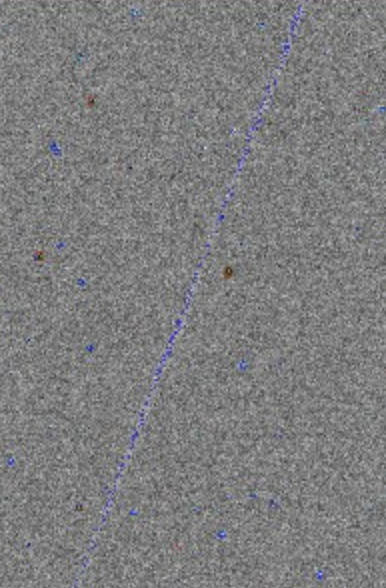
\includegraphics[width=0.5\linewidth]{dia/figures/decam-streak.png}
    \caption{THIS IS DECAM, NOT COMCAM. A typical faint satellite streak in a portion of a difference image where only some regions in the streak fall above the image detection threshold. The streak detection algorithm did not recognize this as a streak, because the regions of the image masked detected (blue) are not contiguous. After binning the image to effectively boost the streak surface brightness, it was readily detected.}
    \label{fig:decam-streak}
\end{figure}
\fi

\subsubsection{Mitigating streaks in DRP}

In most situations, the usual outlier clipping done during coadd assembly with the CompareWarp algorithm excludes streaks from coadds. The coadds where streaks remain all tend to have very few input images, so the streak was not able to be flagged and excluded as an outlier. Work is underway to assess the performance of detecting streaks via the kernel Hough transform in ComCam on top of the standard outlier clipping.

\subsubsection{Mitigating streaks in AP}

Work is underway to detect and masking streaks and glints in difference images. ComCam observations are an important data set for testing how well this works in various situations. A more detailed report will be available in the coming weeks. The efforts described here are distinct from work to identify long trailed sources and cross-check with an external satellite catalog.
